  %% diplomarbeit.tex
  %% Copyright 2015 Simon M. Laube
  %% Update 2022 by Clemens Freudenthaler and Felix Pfahler
  %% Update 2023 by Katja Breitner, Luca Kappel and Mario Hieber for doublesided Print 
  %
  % This work may be distributed and/or modified under the
  % conditions of the LaTeX Project Public License, either version 1.3
  % of this license or (at your option) any later version.
  % The latest version of this license is in
  %   http://www.latex-project.org/lppl.txt
  % and version 1.3 or later is part of all distributions of LaTeX
  % version 2005/12/01 or later.
  %
  % This work has the LPPL maintenance status `author maintained'.
  % 
  % The Current Maintainer of this work is S. M. Laube
  %
  % This work consists of the files listed in ./Help/files.txt

%%=====================================================%%
%% Neues Diplomarbeitstemplate der ET	   			         %%
%% Abteilung ab 2013/2014				   			               %%
%% Erstellt von Simon Michael Laube		   			         %%
%% Betreut von  Prof. Mag. Dipl.-Ing. Dr. Daniel Asch  %%
%%			        Prof. Dipl.-Ing. Dr. Wilhelm Haager	   %%
%%=====================================================%%
%% Dokumentklasse KOMA-Script Report

%% benötigt, da scrpage2 seit KOMA-Script 3.3 (April 2020) als veraltet gilt
%% Philipp Eilmsteiner 17.09.2020
\RequirePackage{scrlfile}
\ReplacePackage{scrpage2}{scrlayer-scrpage}

\documentclass[paper=a4,12pt,pointlessnumbers,twoside]{scrreprt}
%\usepackage[automark]{scrlayer-scrpage} 
% Encoding UTF8
\usepackage[utf8]{inputenc}
% 8 Bit Aufloesung der Buchstaben
\usepackage[T1]{fontenc}
% Seitenraender
\usepackage[scale=0.72]{geometry}
% Spracheinstellungen
\usepackage[english, naustrian]{babel} % your native language must be the last one!!
% erweiterte Farbenpalette
\usepackage[dvipsnames, table]{xcolor}
% Abbildungen
\usepackage{graphicx}
% Tabellen (erweitert)
\usepackage{tabularx}
% TikZ + Circuit-TikZ (fuer Schaltungen)									
\usepackage[europeanresistors,							
			europeaninductors]{circuitikz}
% Nuetzliche TikZ Libraries
\usetikzlibrary{arrows,automata,positioning}
% Mathematikpakete!
\usepackage{amsmath,amssymb}							
%\usepackage{mathtools}	
% PDF Einbindung (zB Datenblaetter)
\usepackage{pdfpages}
% Source Code Einbindung, Setup siehe:
% http://en.wikibooks.org/wiki/LaTeX/Source_Code_Listings									
\usepackage{listings,scrhack} %scrhack vermeidet Umschaltung auf KOMA Floats..			
			
\usepackage{verbatim}
\usepackage{textcomp}

\usepackage{eurosym}
\usepackage{lscape}
% Diplomarbeitsspezifisches Package etdipa
\usepackage{etdipa}

%% Abkuerzungsverzeichnis
\usepackage[]{acronym}

%% Todos
\usepackage[]{todonotes}

%% Ganttdiagramme
\usepackage{pgfgantt}

\usepackage{keyval}
\usepackage{caption}

%% Subfigures
\usepackage[lofdepth]{subfig}

%% HTL-Package (für HTL-Grün)
\usepackage{htlstp}

\usepackage{import}

\usepackage{array}
\usepackage{ragged2e}
\usepackage{csvsimple}

\usepackage{wasysym}
%\usepackage{afterpage}

%\usepackage{pdflscape}
\usepackage{lscape}

\usepackage{setspace}\usepackage{threeparttable}
\usepackage{graphbox} %loads graphicx package
\usepackage[most]{tcolorbox}
\usepackage{multirow}

\usepackage{longtable}

\usepackage{nameref}
\usepackage{arrayjob}
% folowing  must be in this order
\usepackage{varioref}
\usepackage[colorlinks=true,
			linkcolor=black,
			citecolor=black,
			bookmarks=true,
			urlcolor=black,
			bookmarksopen=true]{hyperref}
\usepackage{cleveref}
\usepackage{float}
\usepackage{rotating}
\usepackage{longtable}
\usepackage[numbered,framed]{matlab-prettifier}
%\usepackage[allfiguresdraft]{draftfigure}
\usepackage{enumitem}
\usepackage{pifont}
\usepackage{multicol}
\usepackage{array}

\usepackage{fancyvrb} %Fancy Code-Layout

\newcolumntype{L}[1]{>{\raggedright\let\newline\\\arraybackslash\hspace{0pt}}p{#1}}


\lstset{
  style              = Matlab-editor,
  basicstyle         = \mlttfamily,
  escapechar         = ",
  mlshowsectionrules = true,
}


\RedeclareSectionCommand[beforeskip=0pt]{chapter}

\pdfcompresslevel=9 
\pdfobjcompresslevel=9

%%==== Definitionen fuer die Diplomarbeit ============%%
\dokumenttyp{DIPLOMARBEIT}
\title{Diplomarbeits-Titel}
\author{Max Mustermann \and Martina Musterfrau}
\date{\today}
\place{St. P\"olten}
\schuljahr{2022/23}
\professor{Univ.-Prof. Dr. Albert Einstein \and Univ.-Prof. Dr. Nils Bohr}
\dipacolor{htlgruen}
%%====================================================%%

%% ----------------- define für Leerseiten bei Doppelseitigem-Druck --------------- %%
% 1 aktiv, nicht 0 inaktiv
%\def\emptyprintpages{1}
%\def\emptyprintpages{1}

% Leere Seite mit Kopf- und Fußzeile
\def\blankpage{
	\clearpage
	\null
	\clearpage}

% Leere Seite ohne Kopf- und Fußzeile 
\def\blankemptypage{
	\clearpage
	\thispagestyle{empty}
	\null
	\clearpage}

\begin{document}

\frontmatter
%%================ Titelseite ==========================%%
\maketitle
% Verantwortliche/Verfasser
\responsible{Max Mustermann, Martina Musterfrau}
%%======================================================%%

%%================ Eidesstattliche Erklaerung ==========%%
\begin{Eid}%Unterschrift der Diplomanden hinzufuegen!
\unterschrift{Max Mustermann}
\unterschrift{Martina Musterfrau}
\end{Eid}
%%======================================================%%

\blankpage

%%================ Diplomandenvorstellung ==============%%
%% start of file diplomanden.tex

%% Diplomandenvorstellung:
\begin{Diplomandenvorstellung}
%% Schueler1 
\diplomand{Max Mustermann}
		  {01.03.2002 in St.Pölten}
		  {Waldstraße 3}
		  {3100 St.Pölten}
		  {\schule{2017--2022}{HTBLuVA St.Pölten, Abteilung für Elektrotechnik}
		  \schule{2012--2017}{NMS St. Pölten}}
		  {privat@mail.at}
		  {Images/portraits/bild}
\blankpage
%% Schueler2
\diplomand{Martina Musterfrau}
			{01.01.2002 in St.Pölten}
			{Waldstraße 3}
			{3100 St.Pölten}
			{\schule{2017--2022}{HTBLuVA St.Pölten, Abteilung für Elektrotechnik}
			\schule{2012--2017}{NMS St. Pölten}}
			{privat@mail.at}
			{Images/portraits/bild}
\end{Diplomandenvorstellung}

%% end of file diplomanden.tex

\responsible{Max Mustermann, Martina Musterfrau}
%%======================================================%%
\blankpage

%%================ Danksagungen ========================%%
%% start of file danksagungen.tex

%% Danksagungen:
\begin{Danksagung}
    In der Danksagung kann frei und ohne Vorgabe jeder und jedem gedankt werden, die oder der zum Erfolg der Arbeit beigetragen hat. Sie sollte eine Seite nicht überschreiten.
\end{Danksagung}
\newpage

%% end of file danksagungen.tex
%%======================================================%%
\blankpage

%%================ Abstract /Zusammenfass. =============%%
%% start of file zusammenfassung.tex

\selectlanguage{naustrian}
\renewcommand{\abstractname}{Kurzfassung}
\begin{abstract}
    Die Kurzfassung ist ein sehr wichtiger und der vermutlich am meisten gelesene Teil eines wissenschaftlichen Dokuments.
    
    Es soll auf einer halben Seite der Inhalt der Arbeit zusammengefasst werden. Dabei soll auf die Ausgangslage, das Ziel, die Umsetzung und auch das finale Ergebnis eingegangen werden.
    
    Der Leserin oder dem Leser soll klar sein, was der Inhalt der Arbeit ist, und ob sich ein Lesen der Arbeit für die jeweiligen Recherchezwecke auszahlt. Deswegen ist auch das Ergebnis wichtig.
\end{abstract}
%% end of file zusammenfassung.tex
%% start of file abstract.tex

\selectlanguage{english}
\begin{abstract}
    English version of the Kurzfassung.
\end{abstract}
\selectlanguage{naustrian}

%% end of file abstract.tex
%\selectlanguage{english} % necessary for English speaking users
% delete this line if your native language is German 
%%======================================================%%
\blankpage
%% Beiblaetter
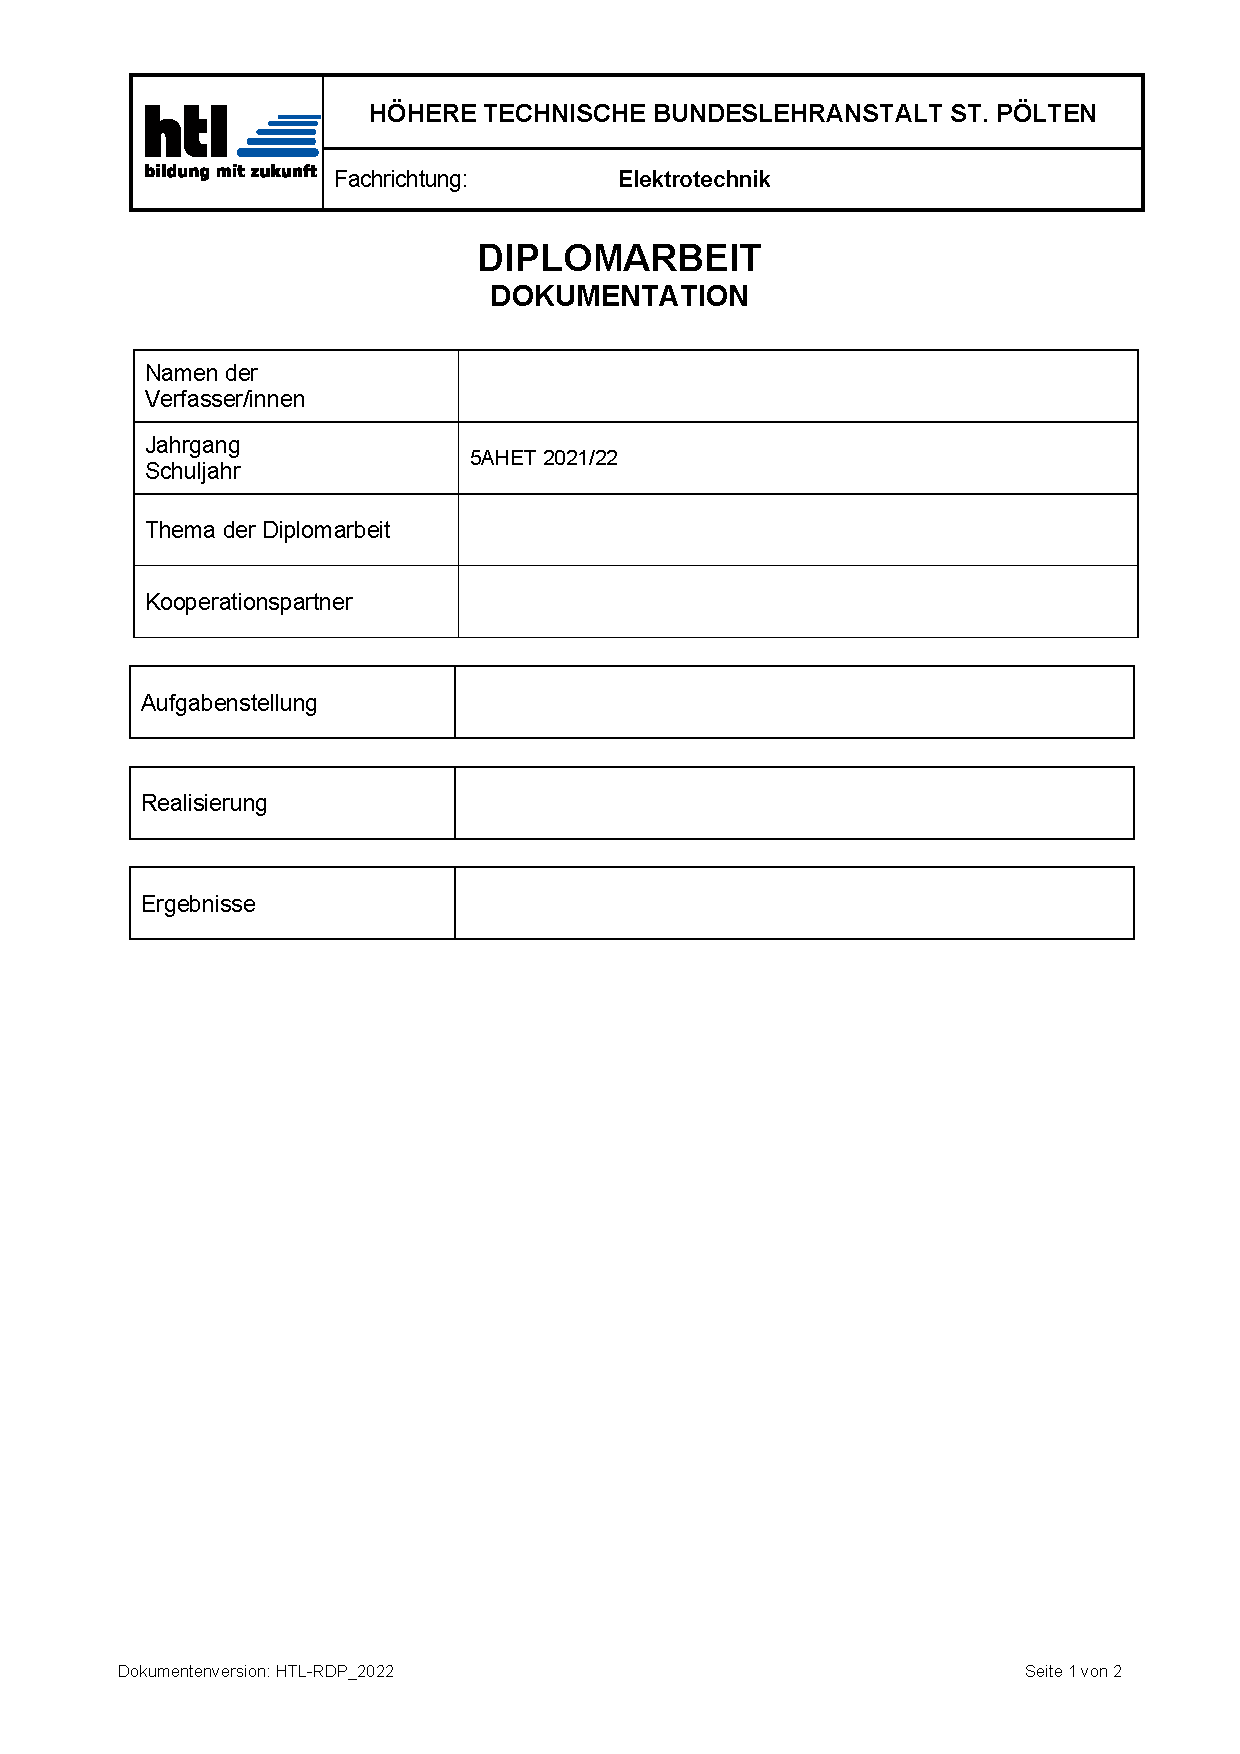
\includepdf[pages={1-2},noautoscale=false,fitpaper=false,scale=0.8, pagecommand={}]{HTL_RDP_Dokumentation_DA_DE_A4_2022.pdf}
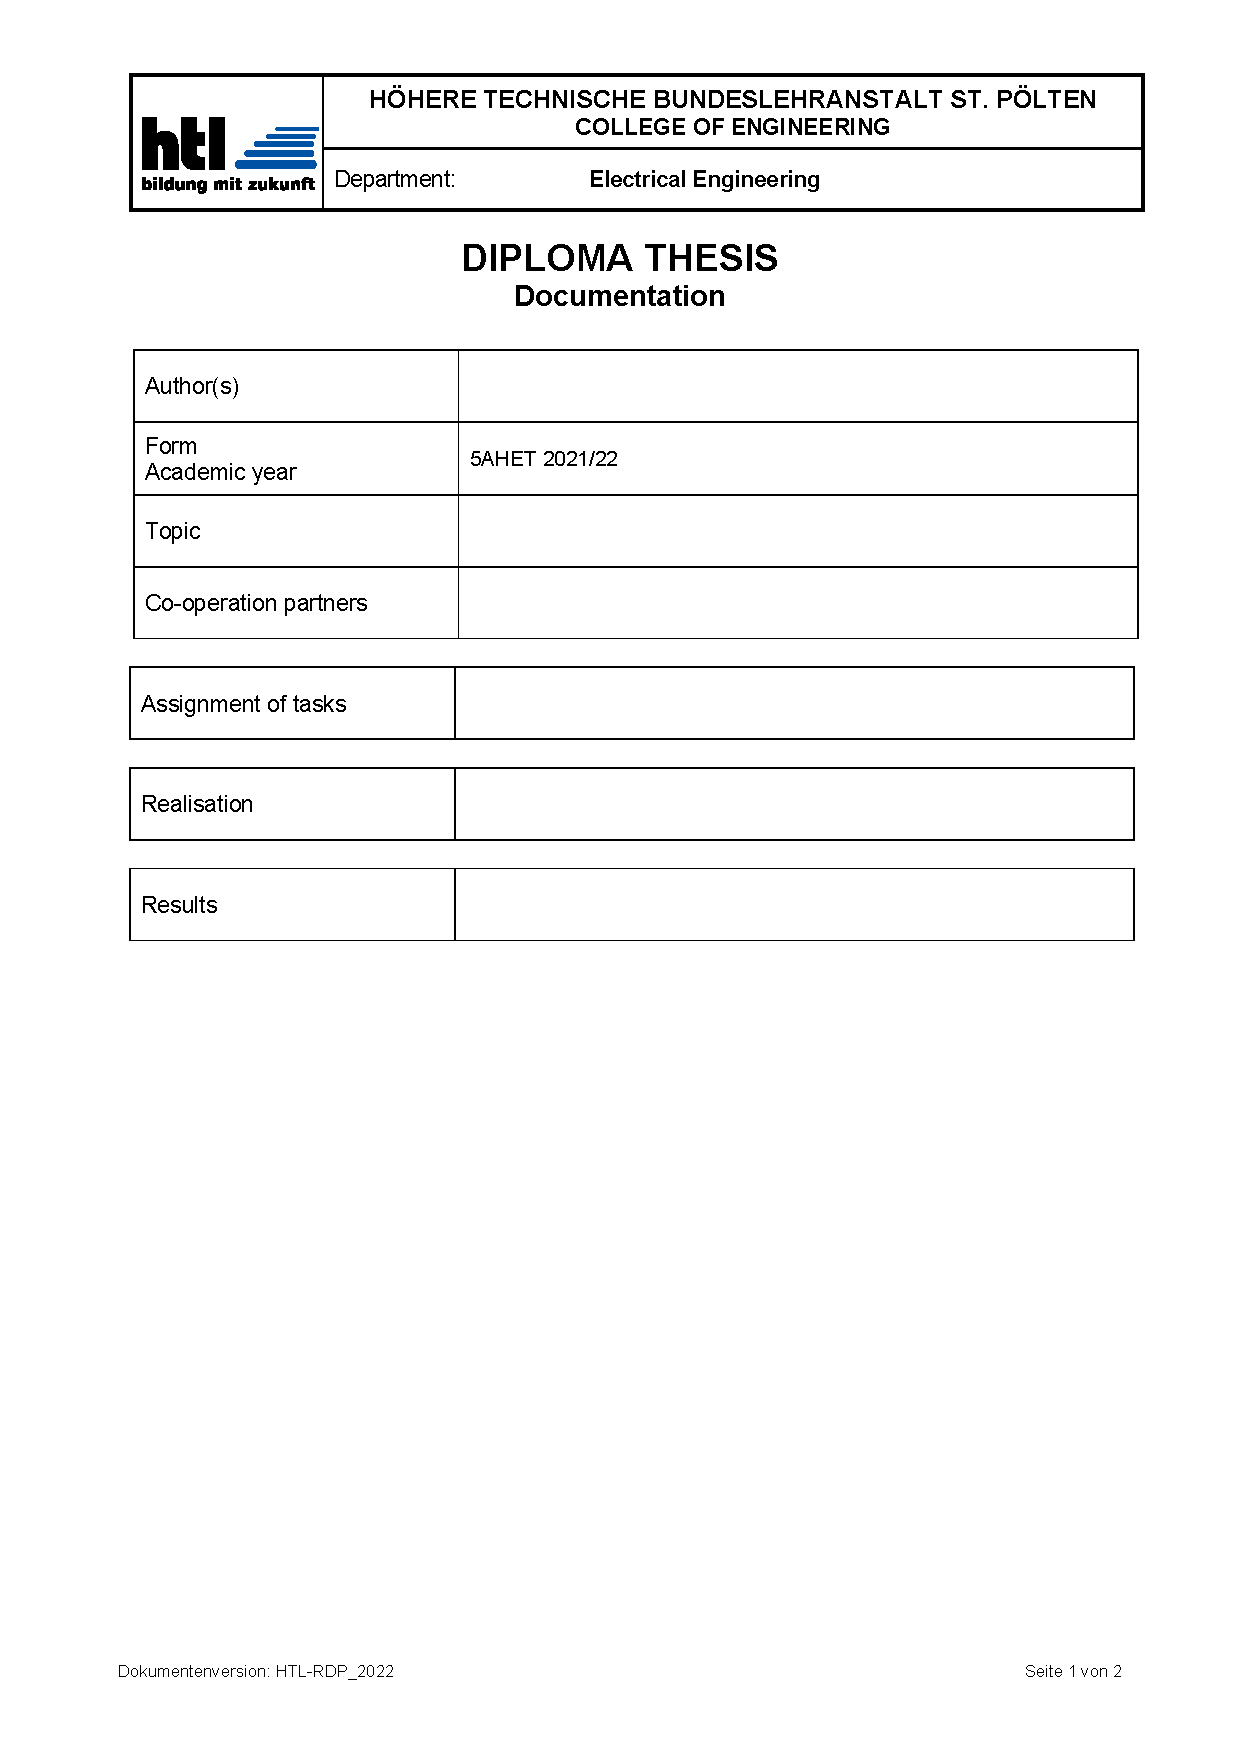
\includepdf[pages={1-2},noautoscale=false,fitpaper=false,scale=0.8, pagecommand={}]{HTL_RDP_Dokumentation_DA_EN_A4_2022.pdf}

%%================ Inhaltsverzeichnis ==================%%
\tableofcontents

%%======================================================%%


% Ab hier Hauptteil
\mainmatter
\blankpage
\chapter{Einleitung}
\responsible{Max Mustermann}
Hier soll eine übersichtliche und einfache Einleitung in wenigen Seiten erfolgen. 
Es kann auf die Ausgangslage, das Konzept und den Bezug zur Praxis eingegangen werden. 
Zitate und Fußnoten sind hier nicht üblich aber nicht verboten.

\chapter{Theoretische Betrachtungen}
\responsible{Martina Musterfrau}

Theoretische Abhandlungen und Literaturrecherche. Es ist wichtig dass die Person die das jeweilige Kapitel verfasst hat davor im \verb|\responsible{}|-Tag angeführt ist. Bitte unbedingt zitieren!

Zitiert kann entweder direkt nach dem einem Absatz werden. Dafür wird am Ende

\section{Referenzieren und Literatur mit \LaTeX}
Prinzipiell gibt es zwei verschiedene Möglichkeiten ein Literaturverzeichnis zu erstellen: Manuell oder automatisch mit Unterstützung eines Hilfsprogrammes. Im folgenden wird das manuelle Erstellen mit der thebibliography-Umgebung erklärt, wie sie in der Diplomarbeitsvorlage angewandt wird. \cite{litKomb}

In der HTL St. Pölten zitieren wir nach dem IEEE-Stil. Wie Einträge im Inhaltsverzeichnis aussehen sollen ist unter folgendem Link nachzulesen:

\url{https://thesius.de/blog/articles/zitieren-ingenieur-ieee-din-iso-690/}

\subsection{Literaturverzeichnis}
Am Ende der Datei wird ein Abschnitt \verb|thebibliography| gesetzt. \verb|thebibliography| enthält die kompletten Informationen zu den Einträgen im Literaturverzeichnis.
\begin{Verbatim}[frame=single]
\begin{thebibliography}{laengste Labelbreite}
	\bibitem[text]{bezugspunkt}
\end{thebibliography}
\end{Verbatim}
In dem Feld \verb|laengste Labelbreite| wird etwas eingetragen, das mindestens so lang ist, wie das längste Label eines Eintrages (eine Zeile darunter).

Das optionale Argument \verb|text| kann ein Label enthalten, welches sowohl im Text als auch im Literaturverzeichnis erscheint.

Der Pflichtparameter \verb|bezugspunkt| enthält eine kurze Bezeichnung des Eintrages. Anhand dieser Bezeichnung wird ein Bezug von dem Verweis im Text zum Literaturverzeichnis erstellt.
\begin{Verbatim}[frame=single]
\begin{thebibliography}{99}
  \bibitem[1]{tietze} U. Tietze und C. Schenk, \textit{Electronic 
    circuits. handbook for design and application.} Heidelberg: 
    Springer, 2015.
  \bibitem[2]{litKomb} Wikibooks. (4.1.21) \textit{LaTeX-Kompendium: 
    Schnellkurs: Erstellen eines Literaturverzeichnisses}. [Online]. 
    Available: \url{https://de.wikibooks.org/wiki/LaTeX-Kompendium:
    \_Schnellkurs:\_Erstellen\_eines\_Literaturverzeichnisses}
\end{thebibliography}
\end{Verbatim}
Im \verb|\bibitem|-Befehl darf kein Zeilenumbruch verwendet werden.

Um die Überschrift des Literaturverzeichnisses zu ändern, kann folgender Befehl verwendet werden:
\begin{Verbatim}[frame=single]
\renewcommand{\refname}{Mein Literaturverzeichnis}
\end{Verbatim}
Das Literaturverzeichnis enthält alle Einträge, egal ob sie benutzt werden, oder nicht (im Gegensatz zu BibTeX, siehe unten).
% ----------------------------------------------------------------------

\subsection{Verweis aus dem Text}
Im Text wird hinter dem Zitat der Befehl \verb|\cite| verwendet.
\begin{Verbatim}[frame=single]
.... Im Grunde besteht kein Unterschied zwischen einem normalen Ver-
starker und einem Operationsverstarker. Beide dienen dazu, Spannungen 
oder Leistungen zu verstärken. \cite[S.~44]{tietze} ...
\end{Verbatim}
Um eine Quelle in das Literaturverzeichnis aufzunehmen, ohne dass sie explizit im Text als Quelle aufgeführt wird, ist \verb|\nocite| zu verwenden.

\nocite{tietze}
%
\chapter{Konstruktion des Prototypen}
\responsible{Max Mustermann}
Hier wird der Entwicklungsvorgang des/der Prototypen penibel genau dokumentiert. 
%

%\chapter{Kostenaufstellung}
%\responsible{Tobias Sturmlechner}
In der nachfolgenden Tabelle \ref{tab:Kosten} sind die Materialkosten, welche im Zuge der Diplomarbeit entstanden sind, aufgelistet. Zwischen privaten und über die Abteilung abgewickelten Bestellungen wird nicht unterschieden. Kostenfrei zur Verfügung gestellte Bauteile und Materialien aus privaten und schulischen Beständen sind ebenfalls nicht aufgelistet.

\begin{longtable}{l|c|c|c}
      {\textbf{Bezeichnung}} & {\textbf{Stück}} & {\textbf{Preis/Stück}} & {\textbf{Gesamt}} \\
      \hline
      \hline
      {Schwingquarz $12\,MHz$} & {5} & {1.64\euro{}} & {8.20\euro{}} \\
      \hline
      {Lochraster Platine} & {3} & {3.85\euro{}} & {11.55\euro{}} \\
      \hline
      {USB-C-Buchse} & {2} & {12.18\euro{}} & {24.36\euro{}} \\
      \hline
      {PCM2906CDB} & {5} & {11.96\euro{}} & {59.80\euro{}} \\
      \hline
      {SSOP28 Adapterplatine} & {3} & {2.38\euro{}} & {7.14\euro{}} \\
      \hline
      {XLR-Buchse} & {2} & {5.72\euro{}} & {11.44\euro{}} \\
      \hline
      {USB-B-Buchse} & {5} & {1.10\euro{}} & {5.49\euro{}} \\
      \hline
      {Klinken Buchse 6.3mm} & {4} & {3.73\euro{}} & {14.92\euro{}} \\
      \hline
      {TLC2274} & {5} & {3.47\euro{}} & {17.35\euro{}} \\
      \hline
      {Buchsenleiste} & {5} & {0.89\euro{}} & {4.45\euro{}} \\
      \hline
      {Stiftleiste} & {5} & {1.02\euro{}} & {5.10\euro{}} \\
      \hline
      {Lötzinn} & {1} & {18.53\euro{}} & {18.53\euro{}} \\
      \hline
      {Doppelpotentiometer $10\,k\Omega$} & {4} & {1.28\euro{}} & {5.12\euro{}} \\
      \hline
      {Doppelpotentiometer $50\,k\Omega$} & {4} & {2.14\euro{}} & {8.56\euro{}} \\
      \hline
      {DRV134PA} & {4} & {6.54\euro{}} & {26.16\euro{}} \\
      \hline
      {INA134PA} & {4} & {3.94\euro{}} & {15.76\euro{}} \\
      \hline
      {Transformator 74010} & {1} & {5.88\euro{}} & {5.88\euro{}} \\
      \hline
      {LM7805} & {5} & {1.80\euro{}} & {9.00\euro{}} \\
      \hline
      {LM7905} & {5} & {1.82\euro{}} & {9.10\euro{}} \\
      \hline
      {XLR-Buchse} & {2} & {4.26\euro{}} & {8.52\euro{}} \\
      \hline
      {USB-C-Buchse} & {1} & {12.18\euro{}} & {12.18\euro{}} \\
      \hline
      {Klinken Buchse 6.3mm} & {10} & {1.06\euro{}} & {10.63\euro{}} \\
      \hline
      {Doppelpotentiometer $10\,k\Omega$} & {2} & {1.28\euro{}} & {2.56\euro{}} \\
      \hline
      {INA134UA} & {3} & {4.36\euro{}} & {13.08\euro{}} \\
      \hline
      {DRV135UA} & {3} & {6.58\euro{}} & {19.74\euro{}} \\
      \hline
      {TLC2274AID} & {5} & {3.13\euro{}} & {15.64\euro{}} \\
      \hline
      {MAX320CSA} & {2} & {2.62\euro{}} & {5.24\euro{}} \\
      \hline
      {XLR-/Klinke Kombibuchse} & {2} & {3.89\euro{}} & {7.78\euro{}} \\
      \hline
      {74HC423D} & {5} & {0.73\euro{}} & {3.65\euro{}} \\
      \hline
      {LED grün, rot} & {3} & {1.27\euro{}} & {3.81\euro{}} \\
      \hline
      {Potentiometer $1\,k\Omega$} & {3} & {6.65\euro{}} & {19.95\euro{}} \\
      \hline
      {TL972} & {5} & {1.00\euro{}} & {5.02\euro{}} \\
      \hline
      {FAN2558S38X} & {10} & {0.21\euro{}} & {2.11\euro{}} \\
      \hline
      {ADA4075-2ARZ} & {4} & {2.38\euro{}} & {9.52\euro{}} \\
      \hline
      {MC34063ACD-TR} & {5} & {0.80\euro{}} & {4.00\euro{}} \\
      \hline
      {Schalter} & {5} & {1.25\euro{}} & {6.23\euro{}} \\
      \hline
      {LED grün} & {5} & {0.20\euro{}} & {1.01\euro{}} \\
      \hline
      {Kondensator $10\,\mu F$/$10\,V$} & {10} & {0.61\euro{}} & {6.14\euro{}} \\
      \hline
      {Keramikkondensator $10\,\mu F$} & {25} & {0.33\euro{}} & {8.25\euro{}} \\
      \hline
      {SMD Quarz $12\,MHz$} & {5} & {1.43\euro{}} & {7.15\euro{}} \\
      \hline
      {Elektrolytkondensator $1\,\mu F$/$20\,V$} & {25} & {0.16\euro{}} & {3.95\euro{}} \\
      \hline
      {Elektrolytkondensator $100\,\mu F$/$16\,V$} & {5} & {1.69\euro{}} & {8.47\euro{}} \\
      \hline
      {Elektrolytkondensator  $220\,\mu F$/$16\,V$} & {5} & {2.34\euro{}} & {11.68\euro{}} \\
      \hline
      {Schottky-Diode} & {20} & {0.37\euro{}} & {7.40\euro{}} \\
      \hline
      {Spule $4.7\,\mu H$} & {10} & {0.31\euro{}} & {3.06\euro{}} \\
      \hline
      {Spule $10\,\mu H$} & {10} & {0.33\euro{}} & {3.29\euro{}} \\
      \hline
      {Spule $33\,\mu H$} & {20} & {0.23\euro{}} & {4.60\euro{}} \\
      \hline
      {Spule $100\,\mu H$} & {5} & {0.19\euro{}} & {0.93\euro{}} \\
      \hline
      {Widerstand $4.7\,k\Omega$/$1\,W$/$1\%$} & {25} & {0.43\euro{}} & {10.68\euro{}} \\
      \hline
      {Doppelpotentiometer $10\,k\Omega$} & {2} & {1.28\euro{}} & {2.56\euro{}} \\
      \hline
      {INA134UA} & {3} & {4.36\euro{}} & {13.08\euro{}} \\
      \hline
      {USB-C Lightning Adapter} & {1} & {4.36\euro{}} & {4.36\euro{}} \\
      \hline
      {18650 Halterung} & {20} & {0.54\euro{}} & {10.70\euro{}} \\
      \hline
      {LM78L12F} & {3} & {0.21\euro{}} & {0.63\euro{}} \\
      \hline
      {LM79L12F} & {3} & {0.25\euro{}} & {0.75\euro{}} \\
      \hline
      {HT4928S} & {10} & {0.36\euro{}} & {3.64\euro{}} \\
      \hline
      {Kondensator $10\,\mu F$/$63\,V$} & {10} & {0.04\euro{}} & {0.41\euro{}} \\
      \hline
      {Kondensator $1\,\mu F$/$63\,V$} & {10} & {0.05\euro{}} & {0.50\euro{}} \\
      \hline
      {MAX743EWE} & {2} & {12.99\euro{}} & {25.98\euro{}} \\
      \hline
      {Kondensator $220\,\mu F$/$63\,V$} & {5} & {1.29\euro{}} & {6.45\euro{}} \\
      \hline
      {Kondensator $330\,\mu F$/$63\,V$} & {3} & {0.49\euro{}} & {1.47\euro{}} \\
      \hline
      {MC14538BDG} & {3} & {0.73\euro{}} & {2.19\euro{}} \\
      \hline
      {JLCPCB Platine} & {1} & {50.64\euro{}} & {50.64\euro{}} \\
      \hline
      {Stempelgummi} & {1} & {18.44\euro{}} & {18.44\euro{}} \\
      \hline
            &       & \textbf{Summe} & \textbf{635.94\euro{}} \\
      \caption{Kostenaufstellung}
    \label{tab:Kosten}%
\end{longtable}%
  

\chapter{Zusammenfassung und Ausblick}
\label{chap:zusammenfassung}
\responsible{Max Mustermann, Martina Musterfrau}

Nomen est omen.

% Ab hier Anhang
\appendix
%\chapter{Bedienungsanleitung}
%\responsible{Clemens Freudenthaler, Tobias Sturmlechner}
Die Audio-Connect-Box ist ein allumfassendes und vielfältiges Audio-Interface. 
Sie findet sowohl im professionellen, als auch im privaten Bereich Anwendung.
Mit ihr ist es möglich, sowohl dynamische als auch Kondensatormikrofone, sowie Geräte mit Line-Ausgang zu verwenden. 
Diese Eingangssignale können mit einem USB-C-Gerät, wie zum Beispiel einem Smartphone oder Computer, aufgenommen werden. 
Ebenfalls können Signale des USB-C-Gerätes über den Output an Lautsprecher,
Kopfhörer oder an ein Mischpult ausgegeben werden.
Sofern kein USB-C-Gerät verbunden ist, kann die Audio-Connect-Box als DI-Box, Mikrofonvorverstärker oder zum Einkoppeln einer Phantomspannung genutzt werden.
\vspace{3cm}
    \begin{figure}[H]
        \centering
        \includegraphics[width=1\textwidth]{Images/konzept/Blockschaltbild.pdf}
        \caption*{Blockschaltbild}
    \end{figure}

\pagebreak

\section{Bedienelemente und Anschlüsse}
\subsection{Vorderseite}
    \begin{figure}[H]
        \centering
        \includegraphics[width=0.9\textwidth]{Images/anhang/Frame-2.eps}
        \caption*{}
    \end{figure}
\begin{multicols}{2}
    \begin{enumerate}
        \item[\ding{202}] \textbf{[ON/OFF] - Schalter}    \\
            Schaltet die Audio-Connect-Box ein / aus. 
            Schalten Sie diesen Schalter ein, wenn Sie die Audio-Connect-Box verwenden wollen.
        \item[\ding{203}] \textbf{[ON/OFF] - Anzeige}    \\
            Leuchtet grün, wenn der Schalter [ON/OFF] gedrückt ist.
        \item[\ding{204}] \textbf{[USB-C] - Anschluss}    \\
            Für den Anschluss an ein unterstütztes USB-C-Gerät.
        \item[\ding{205}] \textbf{[AKKU] - Anzeige}    \\
            Während des Ladens wechselt die \ac{led} abwechselnd jede Sekunde zwischen rot und grün.
            Bei zu geringem Ladestand blinkt die \ac{led} rot. Ist der Akku voll geladen, leuchtet die \ac{led} durchgehend grün.
            Bei Verwendung des Akkus leuchtet die \ac{led} durchgehend rot.
        \item[\ding{206}] \textbf{[POWER SOURCE] - Schalter}    \\
            Schaltet zwischen interner und externer Spannungsversorgung um. 
            Um Spannung über den [USB-C]-Anschluss bereitzustellen, darf der Schalter nicht gedrückt sein.
            Soll der interne Akku verwendet werden, muss sich der Schalter in der gedrückten Stellung befinden.
        \item[\ding{207}] \textbf{[OUTPUT] - Regler}    \\
            Regelt die Lautstärke der Buchsen [LINE] \& [XLR]. 
            An der linken Endposition ist der Ausgangspegel minimal. 
            Durch Drehen nach rechts können Sie die Lautstärke erhöhen.
        \item[\ding{208}] \textbf{[PHONES] - Buchse}    \\
            Diese 6.3mm-Klinkenbuchse dient dem Anschluss eines Stereokopfhörers.
        \item[\ding{209}] \textbf{[PHONES] - Regler}    \\
            Regelt die Lautstärke der Buchse [PHONES]. 
            An der linken Endposition ist der Ausgangspegel minimal. 
            Durch Drehen nach rechts können Sie die Lautstärke erhöhen.
    \end{enumerate}
\end{multicols}

\pagebreak
\subsection{Eingangsseite}
    \begin{figure}[H]
        \centering
        \includegraphics[width=0.8\textwidth]{Images/anhang/Frame-1.eps}
        \caption*{}
    \end{figure}
\begin{multicols}{2}
    \begin{enumerate}
        \item[\ding{202}] \textbf{[48V] - Schalter}    \\
            Schaltet die Phantomspannung für den jeweiligen Kanal ein und aus. Wenn Sie diesen Schalter gedrückt haben, wird das an der jeweiligen Kombibuchse [MIC/LINE] angeschlossene Gerät mit Phantomspannung versorgt. Schalten Sie diesen Schalter nur ein, nachdem Sie an den analogen Eingangsbuchsen phantomgespeiste Geräte wie zum Beispiel ein Kondensatormikrofon angeschlossen haben. Schalten Sie die Phantomspannung immer aus, wenn sie nicht erforderlich ist.
        \item[\ding{203}] \textbf{[MIC/LINE] - Kombibuchsen}    \\
            An dieser Buchse können XLR- und Klinkenstecker (symmetrische/unsymmetrische) wie zum Beispiel Mikrofone und Geräte mit Line-Pegel angeschlossen werden. 
        \item[\ding{204}] \textbf{[GAIN] - Regler}    \\
            Regelt die Vorverstärkung des Eingangssignals der jeweiligen Kombibuchse [MIC/LINE]. 
            An der linken Endposition ist die Verstärkung des Eingangspegels minimal. 
            Durch Drehen nach rechts können Sie die Verstärkung erhöhen.
        \item[\ding{205}] \textbf{[PEGEL] - Anzeigen}    \\
            Leuchten je nach Eingangssignal des jeweiligen Kanals auf. 
            Sobald ein Signal am Eingang anliegt, leuchtet die jeweilige \ac{led} grün.
            Die Anzeigen leuchten orange/rot, kurz bevor der Pegel des Eingangssignals die Verzerrungsgrenze erreicht (Übersteuern).
    \end{enumerate}
\end{multicols}

\pagebreak
\subsection{Ausgangsseite}

    \begin{figure}[H]
        \centering
        \includegraphics[width=0.8\textwidth]{Images/anhang/Frame-3.eps}
        \caption*{}
    \end{figure}
\begin{multicols}{2}
    \begin{enumerate}
        \item[\ding{202}] \textbf{[GROUND LIFT] - Schalter}    \\
            Dieser Schalter trennt die Masseverbindung der Ausgangsbuchsen [XLR 1/2] \& [LINE 1/2] im gedrückten Zustand.
            Bei der Verwendung von unsymmetrischen Klinkensteckern für die Buchsen [LINE 1/2] ist dieser Schalter auf jeden Fall zu lösen.
            Grundsätzlich wird empfohlen, diesen Schalter nicht zu drücken. Bei einem Grundrauschen aufgrund von Einkopplungen auf der Leitung ist das Drücken des Schalters eine mögliche Lösung. Dies ist vom jeweiligen Anwendungsfall abhängig.
        \item[\ding{203}] \textbf{[XLR L/1 \& R/2] - Buchse}    \\
            Zum Anschließen von aktiven Lautsprechern oder
            externen Geräten mit Line-Pegel. An diesen Buchsen
            können XLR-Stecker angeschlossen werden. 
        \item[\ding{204}] \textbf{[LINE L/1] - Buchse}    \\
            Zum Anschließen von aktiven Lautsprechern oder
            externen Geräten mit Line-Pegel. An dieser Buchse
            können 6.3mm-Klinkenstecker (symmetrisch/unsymmetrisch)
            angeschlossen werden. 
            Wenn ausschließlich diese Buchse verwendet wird, wird an dieser ein Mono-Signal des linken und rechten Kanals ausgegeben.
        \item[\ding{205}] \textbf{[LINE R/2] - Buchse}    \\
            Zum Anschließen von aktiven Lautsprechern oder
            externen Geräten mit Line-Pegel. An dieser Buchse
            können 6.3mm-Klinkenstecker (symmetrisch/unsymmetrisch)
            angeschlossen werden.
    \end{enumerate}
\end{multicols}

\pagebreak

\section{Verwendung der Audio-Connect-Box}
\label{sec:anleitung-verwendung}
Der USB-Chip (USB AUDIO CODEC) der \ac{acb} funktioniert über den USB Audio Class 1 Standard.
Deshalb ist keine Installation von Treibern oder zusätzlicher Software nötig. Der USB Audio Class 1 Standard wird von allen modernen Betriebssystemen standardmäßig unterstützt. Bei den meisten Geräten wird ein neu verbundenes Audiogerät sofort als Ein-/Ausgabegerät ausgewählt. Ist dies nicht der Fall, beachten Sie bitte die folgenden, zu Ihrem Betriebssystem passenden, Anweisungen.
\subsection{Windows}

\begin{minipage}[t]{0.55\textwidth}
Unterstützt werden die Betriebssystemversionen Windows 7/8/8.1/10 und Windows 11.
Bei Windows kann die \ac{acb} als Audiogerät in der Taskleiste beim Lautsprechersymbol oder unter \dq Einstellungen > System > Sound\dq\; ausgewählt werden.
\end{minipage}
\begin{minipage}[t]{0.45\textwidth}
    
\begin{figure}[H]
    \centering
    \includegraphics[width=0.8\textwidth]{Images/anhang/windows_taksbar.png}
    \caption*{}
\end{figure}

\end{minipage}
\begin{figure}[H]
    \centering
    \includegraphics[width=0.8\textwidth]{Images/anhang/windows_pref.png}
    \caption*{}
\end{figure}
Die Bitrate und Samplingfrequenz kann unter  \dq Rechtsklick auf Lautsprechersymbol > Sounds > Wiedergabe/Aufnahme > USB AUDIO CODEC > Eigenschaften > Erweitert\dq\; eingestellt werden.
\begin{figure}[H]
    \centering
    \includegraphics[width=0.8\textwidth]{Images/anhang/windows_old.png}
    \caption*{}
\end{figure}

\subsection{MacOS}
\begin{minipage}[t]{0.55\textwidth}
    Die \ac{acb} sollte mit allen Versionen von macOS kompatibel sein, jedoch kann dies nur unter Verwendung von macOS Mojave (10.14) garantiert werden. Bei MacOS kann die \ac{acb} in der Menüleiste beim Lautsprechersymbol oder unter \dq Einstellungen > Ton > Eingabe/Ausgabe\dq\; der USB AUDIO CODEC ausgewählt werden. 
\end{minipage}
\pagebreak
\begin{minipage}[t]{0.45\textwidth}
    \vspace{0pt}
    \centering
    \includegraphics[width=0.8\textwidth]{Images/anhang/mac_bar.png}
\end{minipage}

\begin{figure}[H]
    \centering
    \includegraphics[width=0.7\textwidth]{Images/anhang/mac_preferences.png}
    \caption*{}
\end{figure}
Die Bitrate und Samplingfrequenz kann unter \dq Spotlight-Suche > Audio MIDI Setup.app > USB AUDIO CODEC 1/2\dq\; eingestellt werden.
\begin{figure}[H]
    \centering
    \includegraphics[width=0.7\textwidth]{Images/anhang/mac_audio-midi.png}
    \caption*{}
\end{figure}
\pagebreak
\subsection{Linux}
Die \ac{acb} ist grundsätzlich mit allen gängigen Linux-Distributionen kompatibel, jedoch wurde die korrekte Funktion nur mit Ubuntu 20.4.1 LTS getestet. Bei Linux kann das Audiogerät unter \dq Einstellungen > Sounds > Input/Output\dq\; ausgewählt werden.
\begin{figure}[H]
    \centering
    \includegraphics[width=0.8\textwidth]{Images/anhang/linux.png}
    \caption*{}
\end{figure}

\pagebreak
\subsection{Android}
\begin{minipage}[t]{0.55\textwidth}
Eine Verwendung der \ac{acb} mit Android-Geräten sollte ab Android 5.0 möglich sein, sofern dies durch den jeweiligen Hersteller nicht unterbunden wird. Getestet wurde die korrekte Funktionsweise mit diversen neuen Android-Geräten von Samsung, Google, Motorola und Xiaomi. 
\end{minipage}
\begin{minipage}[t]{0.45\textwidth}
    \vspace{-5pt}
    \centering
    \includegraphics[width=0.8\textwidth]{Images/anhang/Android_music.jpg}
\end{minipage}


\subsection{iOS}
\begin{minipage}[t]{0.55\textwidth}
Bei der Verwendung der \ac{acb} mit iOS-Geräten ist der \dq Lightning auf USB Kamera-Adapter\dq\; notwendig.
Das Audiogerät kann direkt in den jeweiligen Audioapps, wie zum Beispiel in der Musikapp, Spotify oder GarageBand, ausgewählt werden. 
\end{minipage}
\begin{minipage}[t]{0.45\textwidth}
    \vspace{0pt}
    \centering
    \includegraphics[width=0.8\textwidth]{Images/anhang/ios_device.png}
\end{minipage}




\pagebreak

\section{Fehlerbehebung}
\begin{table}[H]
    \centering
    \begin{tabularx}{\textwidth}{|L{4cm}|X|}
        \hline
        \cellcolor[rgb]{ .816,  .808,  .808} \textbf{Das Gerät lässt sich ohne USB-Verbindung nicht einschalten.} & \textbf{Ist der Akku ausreichend geladen?} \newline
            Wurde das Gerät längere Zeit nicht verwendet, besteht die Möglichkeit, dass sich der Akku entladen hat.
            Versuchen Sie den Akku über die USB-C-Buchse zu laden. \\
        \hline
        \cellcolor[rgb]{ .906,  .902,  .902} \textbf{Das Gerät lässt sich mit USB-Verbindung nicht einschalten.} & \textbf{Ist der [POWER SOURCE] - Schalter in der richtigen Position?} \newline
            Überprüfen Sie, ob bei nicht gedrücktem Schalter, das angeschlossene USB-C-Gerät den erforderlichen Strom zur Verfügung stellen kann (Probleme bei Smartphones).
            Überprüfen Sie, ob bei gedrücktem Schalter, der Akku ausreichend geladen ist. \\
        \cline{2-2} \cellcolor[rgb]{ .906,  .902,  .902} & \textbf{Ist das verwendete USB-C-Kabel intakt?} \newline 
            Wenn das USB-C-Kabel gebrochen oder anderweitig beschädigt ist, ersetzen Sie das Kabel durch ein neues. Verwenden Sie kein USB-C-Kabel mit einer Länge von mehr als drei Metern. \\
        \hline
        \cellcolor[rgb]{ .816,  .808,  .808} \textbf{Kein Ton} & \textbf{Ist das Gerät eingeschaltet bzw. wird die Audio-Connect-Box vom USB-C-Gerät erkannt?} \newline
            Ist das Gerät nicht eingeschaltet, ist der volle Funktionsumfang nicht gegeben.
            Wird die Audio-Connect-Box am USB-C-Gerät nicht angeführt, ist die Verbindung nicht aktiv.
            Schalten Sie die Audio-Connect-Box ein und wählen Sie sie am USB-C-Gerät aus.\\
        \cline{2-2} \cellcolor[rgb]{ .816,  .808,  .808} & \textbf{Sind die Lautstärkeregler des Geräts auf geeignete Pegel eingestellt?} \newline
            Prüfen Sie die Pegel der Drehregler [OUTPUT] und [PHONES]. \\
        \cline{2-2} \cellcolor[rgb]{ .816,  .808,  .808} & \textbf{Sind die Mikrofone, Lautsprecher oder Kopfhörer korrekt am Gerät angeschlossen?} \newline
            Überprüfen Sie die korrekte Verbindung der angeschlossenen Geräte. \\
        \hline
    \end{tabularx}%
\end{table}%
  
\pagebreak

\begin{table}[H]
    \centering
    \begin{tabularx}{\textwidth}{|L{4cm}|X|}
        \hline
        \cellcolor[rgb]{ .906,  .902,  .902}  \textbf{Ungewöhnlicher Klang, Rauschen, Verzerrungen} & \textbf{Leuchtet die [PEGEL] - Anzeige am verwendeten Eingang orange/rot?} \newline
            Das Signal ist zu nahe oder über der Verzerrungsgrenze und kann nicht mehr richtig verarbeitet werden (Übersteuern).
            Regeln Sie die Eingangsverstärkung zurück. \\
        \cline{2-2}   \cellcolor[rgb]{ .906,  .902,  .902}       & \textbf{Liegt ein dauerhaftes Grundrauschen am Ausgabegerät an?} \newline
            Das Einkoppeln von anderen Signalen oder Störungen - vor allem bei langen Leitungen - kann zu diesem Rauschen führen.
            Das Betätigen des [GROUND LIFT] - Schalters kann zur Lösung des Problems beitragen. \\
        \cline{2-2}   \cellcolor[rgb]{ .906,  .902,  .902}       & \textbf{Wurde die Audio-Connect-Box am USB-C-Gerät richtig konfiguriert?} \newline
            Überprüfen Sie die eingestellte Bitrate und Abtastfrequenz und passen Sie diese gegebenenfalls an (siehe Kapitel \ref{sec:anleitung-verwendung}) \\
        \hline
    \end{tabularx}%
\end{table}%
  



\chapter{Besprechungsprotokolle}
\begin{table}[H]
    \begin{tabularx}{\textwidth}{m{3cm}|m{3cm}|l|m{5.5cm}}
    \textbf{Anwesende Schüler} & \textbf{Anwesender Betreuer} & \textbf{Datum} & \textbf{Inhalt} \\ \hline \hline
    Mustermann, Musterfrau & Einstein, Bohr & 06.05.2021 & Ideenfindung \& Organisation \\    \hline       
    Mustermann, Musterfrau & Einstein  & 02.06.2021 & Spannungsversorgung \& \newline 1. Bestellung \\    \hline       
    Mustermann, Musterfrau &  Bohr  & 24.06.2021 & Organisatorisches \& \newline 2. Bestellung \\   \hline        
    Mustermann & Bohr  & 25.06.2021 & Anfrage zweiter \newline Betreuungslehrer \\    \hline       
    Mustermann, Musterfrau & Einstein, Bohr  & 11.11.2021 & Eingangsschaltung \\       \hline    
    Mustermann, Musterfrau & Einstein  & 12.11.2021 & Schaltungsoptimierung \\    \hline       
    Musterfrau & Einstein, Bohr  & 18.01.2022 & Platinenentwurf fertig \& \newline 4. Bestellung \\    \hline
    Mustermann, Musterfrau & Einstein, Bohr  & 04.02.2022 & Fertigungsmöglichkeiten \newline für Gehäuse \\  \hline
    Mustermann, Musterfrau & Einstein, Bohr  & 16.03.2022 & Strombegrenzung \& \newline Dokumentationsstruktur \\
    \end{tabularx}
\end{table}

\vfill
	\begin{table}[h!]
		\hfill
		\begin{tabular}{c}%
		\hline
		Bestätigung der Betreuer
		\end{tabular}
	\end{table}
	\vfill%vertikales Zentrieren

\chapter{Zeitaufstellung}
\section{Max Mustermann}
\begin{longtable}{c|p{10cm}|c}
    \textbf{Datum} & \textbf{Tätigkeit}                                                                                            & \textbf{Stunden} \\ \hline \hline
    06.05.21       & Organisation Diplomarbeit, Ideenfindung                                                                       & 5                \\ \hline
    01.06.21       & erster Prototyp mit USB-Audio-Codec fertig                                                                    & 3                \\ \hline
    02.06.21       & erweiterung für iPhone mit Adapter, Strommessung                                                              & 2                \\ \hline
    02.06.21       & Besprechung: Spannungsversorgung, \newline 1. Bestellliste begonnen                                           & 2.5              \\ \hline
    04.06.21       & Headphone Amp v1 auf Breadboard                                                                               & 1.5              \\ \hline
    07.06.21       & Headphone Amp zusätzliche Stromstütze für Bässe, \newline neuer   Klinkenadapter                              & 1                \\ \hline
    24.06.21       & Besprechung: DB, Spgversorgung, \newline zweiter Lehrer, 2. Bestellung                                        & 0.5              \\ \hline
    25.06.21       & 2. Bestellung fertig gestellt                                                                                 & 1                \\ \hline
    25.06.21       & Besprechung: Anfrage \newline zweiter Betreuungslehrer (FL. Binder)                                           & 0.5              \\ \hline
    02.07.21       & Octaveskript für Oszilloskop                                                                                  & 4                \\ \hline
    08.07.21       & Ausgangsschaltung am Breadboard fertig                                                                        & 4                \\ \hline
    18.07.21       & Schaltung zeichnen Ausgang                                                                                    & 0.5              \\ \hline
    19.07.21       & Eingangsschaltung, clipping LEDs, \newline Ausgang Klinke \& XLR                                              & 4                \\ \hline
    06.11.21       & Fehlersuche Kopfhörerverstärker \newline Lochrasterplatine (Fehler in   Aufbau)                               & 0.5              \\ \hline
    07.11.21       & Fehlersuche Kopfhörerverstärker \newline Lochrasterplatine (Ungleiche   Spannungsversorgung)                  & 0.5              \\ \hline
    08.11.21       & Kopfhörerverstärker repariert (Poti getauscht)                                                                & 2                \\ \hline
    10.11.21       & Besprechung: Platine, Spannungsversorgung                                                                     & 1                \\ \hline
    10.11.21       & Eingangsschaltung Tests                                                                                       & 5                \\ \hline
    10.11.21       & Schaltungsentwurf, 3. Bestellliste schreiben                                                                  & 2                \\ \hline
    11.11.21       & Komparator NE555 organisiert                                                                                  & 0.5              \\ \hline
    11.11.21       & Klinkenstecker Footprintdesign                                                                                & 1                \\ \hline
    11.11.21       & Besprechung: Eingangsschaltung                                                                                & 0.5              \\ \hline
    11.11.21       & Eingangschaltung Entwurf                                                                                      & 1.5              \\ \hline
    12.11.21       & Besprechung: Schaltungsoptimierung                                                                            & 4                \\ \hline
    14.11.21       & SMD-Bauteile gewählt                                                                                          & 2                \\ \hline
    14.11.21       & Kopfhörerverstärker auf Platine gezeichnet                                                                    & 2                \\ \hline
    14.11.21       & Ausgangsschaltung PCB geroutet                                                                                & 2.5              \\ \hline
    25.11.21       & Digitalspannung und Masse getrennt und getestet                                                               & 6                \\ \hline
    25.11.21       & Bootstrapschaltung gezeichnet und simuliert                                                                   & 1.5              \\ \hline
    01.12.21       & Simulation Bootstrap                                                                                          & 1                \\ \hline
    04.12.21       & Bootstrapschaltung fertig simuliert und in Schaltung \newline adaptiert, Planung Spannungsversorgung begonnen & 3                \\ \hline
    05.12.21       & Schaltungsentwurf Spannungsversorgung, \newline 4. Bestellliste   begonnen                                    & 4.5              \\ \hline
    06.12.21       & Spannungsversorgung                                                                                           & 3                \\ \hline
    07.12.21       & Besprechung: Spannungsversorgung, 4. Bestellliste                                                             & 4                \\ \hline
    10.12.21       & Bestellliste SMD aktualisiert, USB-C Android getestet                                                         & 3.5              \\ \hline
    13.12.21       & Platine linker Eingang, Spannungsversorgung                                                                   & 3.5              \\ \hline
    22.12.21       & Problem mit Phantomspeisung (unsymmetrischer \newline Input), Problem   Mono Output besprochen                & 2                \\ \hline
    26.12.21       & Platine Kondensatoren adaptiert                                                                               & 3.5              \\ \hline
    05.01.22       & Platine Digitalschaltung                                                                                      & 1.5              \\ \hline
    08.01.22       & Platine Spannungsversorgung                                                                                   & 2                \\ \hline
    10.01.22       & Platine Beschriftung und Platzierung                                                                          & 1                \\ \hline
    10.01.22       & Bauteilliste ergänzt und überprüft                                                                            & 2                \\ \hline
    14.01.22       & Bauteilliste fertig ergänzt + 4. Bestellliste fertig                                                          & 2                \\ \hline
    14.01.22       & Footprints auf 4. Bestellliste angepasst                                                                      & 1.5              \\ \hline
    17.01.22       & Footprints Eingangsschaltung angepasst (großes C)                                                             & 1                \\ \hline
    17.01.22       & Massefläche                                                                                                   & 2                \\ \hline
    18.01.22       & Besprechung fertiger Print, 4. Bestelliste                                                                    & 1                \\ \hline
    18.01.22       & 4. Bestellliste \& Footprints adaptiert                                                                       & 2                \\ \hline
    19.01.22       & Platine finalisiert, Infos über Bestellung eingeholt                                                          & 2.5              \\ \hline
    20.01.22       & LCSC \& JLCPCB bestellung abgefertig                                                                          & 1                \\ \hline
    25.01.22       & "Fehler" in Bootstrapsimulation gesucht                                                                       & 0.5              \\ \hline
    30.01.22       & Vertrautmachen mit der Diplomarbeitsvorlage, \newline CPE-Besprechnung   5BHET angeschaut                     & 2.5              \\ \hline
    31.01.22       & GitHub für Doku eingerichtet, \newline Diplomantenvorstellung Clemens                                         & 1.5              \\ \hline
    01.02.22       & Verwendung von Git etabliert                                                                                  & 2                \\ \hline
    02.02.22       & Doku: Grundstruktur \& Themenvorstellung                                                                      & 3                \\ \hline
    02.02.22       & Erster Gehäuseentwurf in Fusion 360                                                                           & 1.5              \\ \hline
    04.02.22       & Besprechung: Gehäuse Fertigung                                                                                & 1                \\ \hline
    04.02.22       & Gehäuse bemaßt                                                                                                & 3                \\ \hline
    08.02.22       & Doku: Analoge Oszilloskope, \newline Meilensteine, Besprechungsproktoll                                       & 4                \\ \hline
    12.02.22       & Doku: Gehäuse 3D \& Konstruktionspläne \& Aufdruck                                                            & 1.5              \\ \hline
    16.02.22       & Oszi-Skript überarbeitet, Platine bestückt                                                                    & 8                \\ \hline
    17.02.22       & Platine fertig bestückt                                                                                       & 3                \\ \hline
    18.02.22       & Fehler auf Platine fixen, Platinendesign anpassen                                                             & 5                \\ \hline
    20.02.22       & Gehäuse \& Kappen neu modelliert und dokumentiert                                                             & 7                \\ \hline
    21.02.22       & OPV-Eingangsbeschaltung Korrektur                                                                             & 4                \\ \hline
    21.02.22       & Pläne von Fusionmodelle vorläufig fertig, \newline Kappen 3D-gedruckt                                         & 2                \\ \hline
    22.02.22       & 3D-Kappen probiert, adaptiert und v2 gedruckt                                                                 & 1.5              \\ \hline
    22.02.22       & Fehler bei Eingangsschaltung bearbeiten                                                                       & 3                \\ \hline
    22.02.22       & Beschriftung in Fusion gezeichnet                                                                             & 2                \\ \hline
    23.02.22       & Input repariert, Clipping LED repariert                                                                       & 3.5              \\ \hline
    25.02.22       & Arbeiten an Platine                                                                                           & 6                \\ \hline
    26.02.22       & Doku: Gehäuse, Platine                                                                                        & 3                \\ \hline
    01.03.22       & Doku: Platine, Oszi fotografiert \& platine monoflop fix                                                      & 2                \\ \hline
    02.03.22       & Tests für Einschaltstrombegrenzung \& Kartonmodell \newline für Gehäuse \& Fotos bearbeitet                   & 7                \\ \hline
    03.03.22       & Doku: Kapitel Platine fertig                                                                                  & 2                \\ \hline
    04.03.22       & Doku: Aufdrucke \& Datenblätter eingebungen                                                                   & 2                \\ \hline
    06.03.22       & Doku: Beschriftung als PDF eingebunden                                                                        & 0.5              \\ \hline
    07.03.22       & Doku: Danksagung, Kurzfassung/Abstract fertig                                                                 & 3                \\ \hline
    09.03.22       & Doku: Konzept fertig                                                                                          & 1.5              \\ \hline
    10.03.22       & Doku: Betriebsanleitung                                                                                       & 4                \\ \hline
    16.03.22       & Besprechung: Dokustruktur \& Strombegrenzung                                                                  & 0.5              \\ \hline
    16.03.22       & Gehäuseteile mit Laser schneiden                                                                              & 1.5              \\ \hline
    17.03.22       & Gehäuse gebohrt \& gebogen                                                                                    & 1.5              \\ \hline
    18.03.22       & Gehäuse gebogen \& lackiert                                                                                   & 3.5              \\ \hline
    20.03.22       & Doku: Arbeitsplatz                                                                                            & 0.5              \\ \hline
    21.03.22       & Gehäuse: Gewinde gebohrt, Stempeltests                                                                        & 1.5              \\ \hline
    23.03.22       & Doku: Fehler und Probleme                                                                                     & 4.5              \\ \hline
    23.03.22       & 3D-Model mit Steckermodellen erweitert, \newline Skizzen für   Betriebsanleitung                              & 2.5              \\ \hline
    24.03.22       & Doku: Betriebsanleitung mit Screenshots fertig                                                                & 4.5              \\ \hline
    25.03.22       & Doku: Fehler fertig, Messungen, \newline Laserversuch Moosgummi, Zeitaufstellung eingebunden                  & 7                \\ \hline
    26.03.22       & Plots von Messungen erstellt & 2 \\ \hline
    26.03.22       & Doku: Frequenzgänge der Platine \& Zeichnungen fertig & 4 \\ \hline
    28.03.22       & Dokumentation finalisiert & 6 \\ \hline
    & \multicolumn{1}{r|}{\textbf{Summe}} &   \textbf{239.5} \\

    \caption{Zeitaufstellung Mustermann}
    \label{tab:zeit_clee}
\end{longtable}
\pagebreak
\section{Martina Musterfrau}
\begin{longtable}{c|p{10cm}|c}
    \textbf{Datum} & \textbf{Tätigkeit}                                                                                     & \textbf{Stunden} \\ \hline \hline
    06.05.21       & Organisation Diplomarbeit, Ideenfindung                                                                & 5                     \\ \hline
    01.06.21       & erster Prototyp mit USB-Audio-Codec fertig                                                             & 3                     \\ \hline
    02.06.21       & erweiterung für iPhone mit Adapter, Strommessung                                                       & 2                     \\ \hline
    02.06.21       & Besprechung: Spannungsversorgung, \newline 1. Bestellliste begonnen                                             & 2.5                   \\ \hline
    04.06.21       & Headphone Amp v1 auf Breadboard                                                                        & 1.5                   \\ \hline
    07.06.21       & Headphone Amp zusätzliche Stromstütze für Bässe, \newline neuer   Klinkenadapter                                & 1                     \\ \hline
    24.06.21       & Besprechung: DB, Spgversorgung, \newline zweiter Lehrer, 2. Bestellung                                          & 0.5                   \\ \hline
    25.06.21       & 2. Bestellung fertig gestellt                                                                          & 1                     \\ \hline
    25.06.21       & Besprechung: Anfrage zweiter \newline Betreuungslehrer (FL. Binder)                                             & 0.5                   \\ \hline
    08.07.21       & Ausgangsschaltung am Breadboard fertig                                                                 & 4                     \\ \hline
    17.07.21       & Schaltung zeichnen Kopfhörerverstärker                                                                 & 1.5                   \\ \hline
    18.07.21       & Schaltung zeichnen Ausgang                                                                             & 0                     \\ \hline
    19.07.21       & Eingangsschaltung, clipping LEDs, \newline Ausgang Klinke \& XLR                                                & 4                     \\ \hline
    06.11.21       & Fehlersuche Kopfhörerverstärker \newline Lochrasterplatine (Fehler in   Aufbau)                                 & 0.5                   \\ \hline
    08.11.21       & Kopfhörerverstärker repariert (Poti getauscht)                                                         & 2                     \\ \hline
    10.11.21       & Besprechung: Platine, Spannungsversorgung                                                              & 1                     \\ \hline
    10.11.21       & Eingangsschaltung Tests                                                                                & 5                     \\ \hline
    11.11.21       & Komparator NE555 organisiert                                                                           & 0.5                   \\ \hline
    11.11.21       & Besprechung: Eingangsschaltung                                                                         & 0.5                   \\ \hline
    11.11.21       & Eingangschaltung Entwurf                                                                               & 4                     \\ \hline
    12.11.21       & Besprechung: Schaltungsoptimierung                                                                     & 3.5                   \\ \hline
    13.11.21       & Eingangsschaltung angepasst                                                                            & 1                     \\ \hline
    14.11.21       & SMD-Bauteile gewählt                                                                                   & 2                     \\ \hline
    14.11.21       & Ausgangsschaltung PCB geroutet                                                                         & 2.5                   \\ \hline
    25.11.21       & Digitalspannung und Masse getrennt und getestet                                                        & 6                     \\ \hline
    25.11.21       & Bootstrapschaltung gezeichnet und simuliert                                                            & 1                     \\ \hline
    04.12.21       & Bootstrapschaltung fertig simuliert und in Schaltung \newline adaptiert, Planung Spannungsversorgung begonnen & 3                     \\ \hline
    05.12.21       & Schaltungsentwurf Spannungsversorgung, \newline 4. Bestellliste   begonnen                                      & 4.5                   \\ \hline
    06.12.21       & Spannungsversorgung                                                                                    & 3                     \\ \hline
    07.12.21       & Besprechung: Spannungsversorgung, 4. Bestellliste                                                      & 4                     \\ \hline
    10.12.21       & Bestellliste SMD aktualisiert, USB-C Android getestet                                                  & 3                     \\ \hline
    13.12.21       & Platine linker Eingang, Spannungsversorgung                                                            & 3                     \\ \hline
    22.12.21       & Problem mit Phantomspeisung (unsymmetrischer \newline Input), Problem   Mono Output besprochen                  & 2                     \\ \hline
    23.12.21       & Platine rechter Eingang                                                                                & 3                     \\ \hline
    26.12.21       & Platine Kondensatoren adaptiert                                                                        & 3.5                   \\ \hline
    05.01.22       & Platine Digitalschaltung                                                                               & 1.5                   \\ \hline
    08.01.22       & Platine Spannungsversorgung                                                                            & 2                     \\ \hline
    10.01.22       & Platine Beschriftung und Platzierung                                                                   & 1                     \\ \hline
    10.01.22       & Bauteilliste ergänzt und überprüft                                                                     & 2                     \\ \hline
    14.01.22       & Bauteilliste fertig ergänzt + 4. Bestellliste fertig                                                   & 2                     \\ \hline
    14.01.22       & Footprints auf 4. Bestellliste angepasst                                                               & 0.5                   \\ \hline
    17.01.22       & Footprints Eingangsschaltung angepasst (großes C)                                                      & 1                     \\ \hline
    17.01.22       & Massefläche                                                                                            & 2                     \\ \hline
    18.01.22       & Besprechung fertiger Print, 4. Bestelliste                                                             & 1                     \\ \hline
    18.01.22       & 4. Bestellliste \& Footprints adaptiert                                                                & 2                     \\ \hline
    19.01.22       & Platine finalisiert, Infos über Bestellung eingeholt                                                   & 2.5                   \\ \hline
    20.01.22       & LCSC \& JLCPCB bestellung abgefertig                                                                   & 1                     \\ \hline
    30.01.22       & Vertrautmachen mit der Diplomarbeitsvorlage, \newline CPE-Besprechnung   5BHET angeschaut                       & 2.5                   \\ \hline
    01.02.22       & Verwendung von Git etabliert                                                                           & 2                     \\ \hline
    02.02.22       & Doku: Grundstruktur \& Themenvorstellung                                                               & 3                     \\ \hline
    02.02.22       & Erster Gehäuseentwurf in Fusion 360                                                                    & 0.5                   \\ \hline
    04.02.22       & Besprechung: Gehäuse Fertigung                                                                         & 1                     \\ \hline
    04.02.22       & Gehäuse bemaßt                                                                                         & 2                     \\ \hline
    16.02.22       & Breadboard-Prototypen Fotografieren                                                                    & 4                     \\ \hline
    16.02.22       & Platine bestückt                                                                                       & 4                     \\ \hline
    17.02.22       & Platine fertig bestückt                                                                                & 2                     \\ \hline
    21.02.22       & OPV-Eingangsbeschaltung Korrektur                                                                      & 4                     \\ \hline
    22.02.22       & 3D-Kappen probiert, adaptiert und v2 gedruckt                                                          & 1                     \\ \hline
    23.02.22       & Input repariert, Clipping LED repariert                                                                & 3.5                   \\ \hline
    25.02.22       & Arbeiten an Platine                                                                                    & 6                     \\ \hline
    27.02.22       & Schematics für Export adaptiert                                                                        & 3                     \\ \hline
    01.03.22       & Doku: Platine, Oszi fotografiert \& platine monoflop fix                                               & 2                     \\ \hline
    02.03.22       & Tests für Einschaltstrombegrenzung \& Kartonmodell \newline für Gehäuse \& Fotos bearbeitet                   & 6.5                   \\ \hline
    04.03.22       & Gehäuse, Oberflächenbehandlung                                                                         & 2                     \\ \hline
    07.03.22       & Doku: Danksagung, Kurzfassung/Abstract fertig                                                          & 2.5                   \\ \hline
    09.03.22       & Doku: Konzept fertig                                                                                   & 1.5                   \\ \hline
    09.03.22       & Schematics: Schriftköpfe und Schaltungen angepasst                                                     & 1                     \\ \hline
    09.03.22       & Doku: Schaltung                                                                                        & 1                     \\ \hline
    10.03.22       & Doku: Betriebsanleitung                                                                                & 4                     \\ \hline
    11.03.22       & Schematics für Export adaptiert                                                                        & 2.5                   \\ \hline
    11.03.22       & Doku: Schaltung                                                                                        & 1                     \\ \hline
    12.03.22       & Doku: Schaltung                                                                                        & 1                     \\ \hline
    13.03.22       & Doku: Schaltung                                                                                        & 3.5                   \\ \hline
    16.03.22       & Besprechung: Dokustruktur \& Strombegrenzung                                                           & 0.5                   \\ \hline
    16.03.22       & Gehäuseteile mit Laser schneiden                                                                       & 1.5                   \\ \hline
    16.03.22       & Doku: Quellen angepasst, \newline Schaltung: Kopfhörerverstärker                                                & 1                     \\ \hline
    17.03.22       & Gehäuse gebohrt \& gebogen                                                                             & 1.5                   \\ \hline
    18.03.22       & Gehäuse gebogen \& lackiert                                                                            & 3.5                   \\ \hline
    21.03.22       & Doku: Foto eingefügt, Schaltung: Spannungsversorgung                                                   & 1                     \\ \hline
    21.03.22       & Gehäuse: Gewinde gebohrt, Stempeltests                                                                 & 1                     \\ \hline
    22.03.22       & Schematics angepasst und exportiert                                                                    & 0.5                   \\ \hline
    22.03.22       & Doku: Schaltung                                                                                        & 2.5                   \\ \hline
    23.03.22       & Doku: Fehler und Probleme                                                                              & 4.5                   \\ \hline
    23.03.22       & Doku: Schaltung, Prototypen                                                                            & 4.5                   \\ \hline
    24.03.22       & Doku: Betriebsanleitung mit Screenshots fertig                                                         & 4                     \\ \hline
    25.03.22       & Doku: Fehler fertig, Messungen, \newline Laserversuch Moosgummi                                                 & 6                     \\ \hline
    25.03.22       & Doku: Schaltung & 2 \\ \hline
    25.03.22       & Plots von Messungen erstellt & 1 \\ \hline
    26.03.22       & Plots von Messungen erstellt & 2.5 \\ \hline
    26.03.22       & Doku: Prototypen & 4.5 \\ \hline
    27.03.22       & Doku: Kostenaufstellung & 1 \\ \hline
    28.03.22       & Dokumentation finalisiert & 6 \\ \hline
        & \multicolumn{1}{r|}{\textbf{Summe}} &   \textbf{219.5} \\
    \caption{Zeitaufstellung Musterfrau}
    \label{tab:zeit_tobi}
\end{longtable}


\chapter{Skript Oszilloskop}
\lstinputlisting[style=Matlab-editor, caption=m-Skript für das Auslesen des Oszilloskops, captionpos=b]{Images/analogOszi/ReadOszi.m}
\label{listing:osziskript}
%
%\chapter{Stückliste}
%\label{chap:stueckliste}
%\input{Textparts/main/stueckliste.tex}
%
%\chapter{Datenblätter}
% chapter in include weil wegen inputpdf scheisse

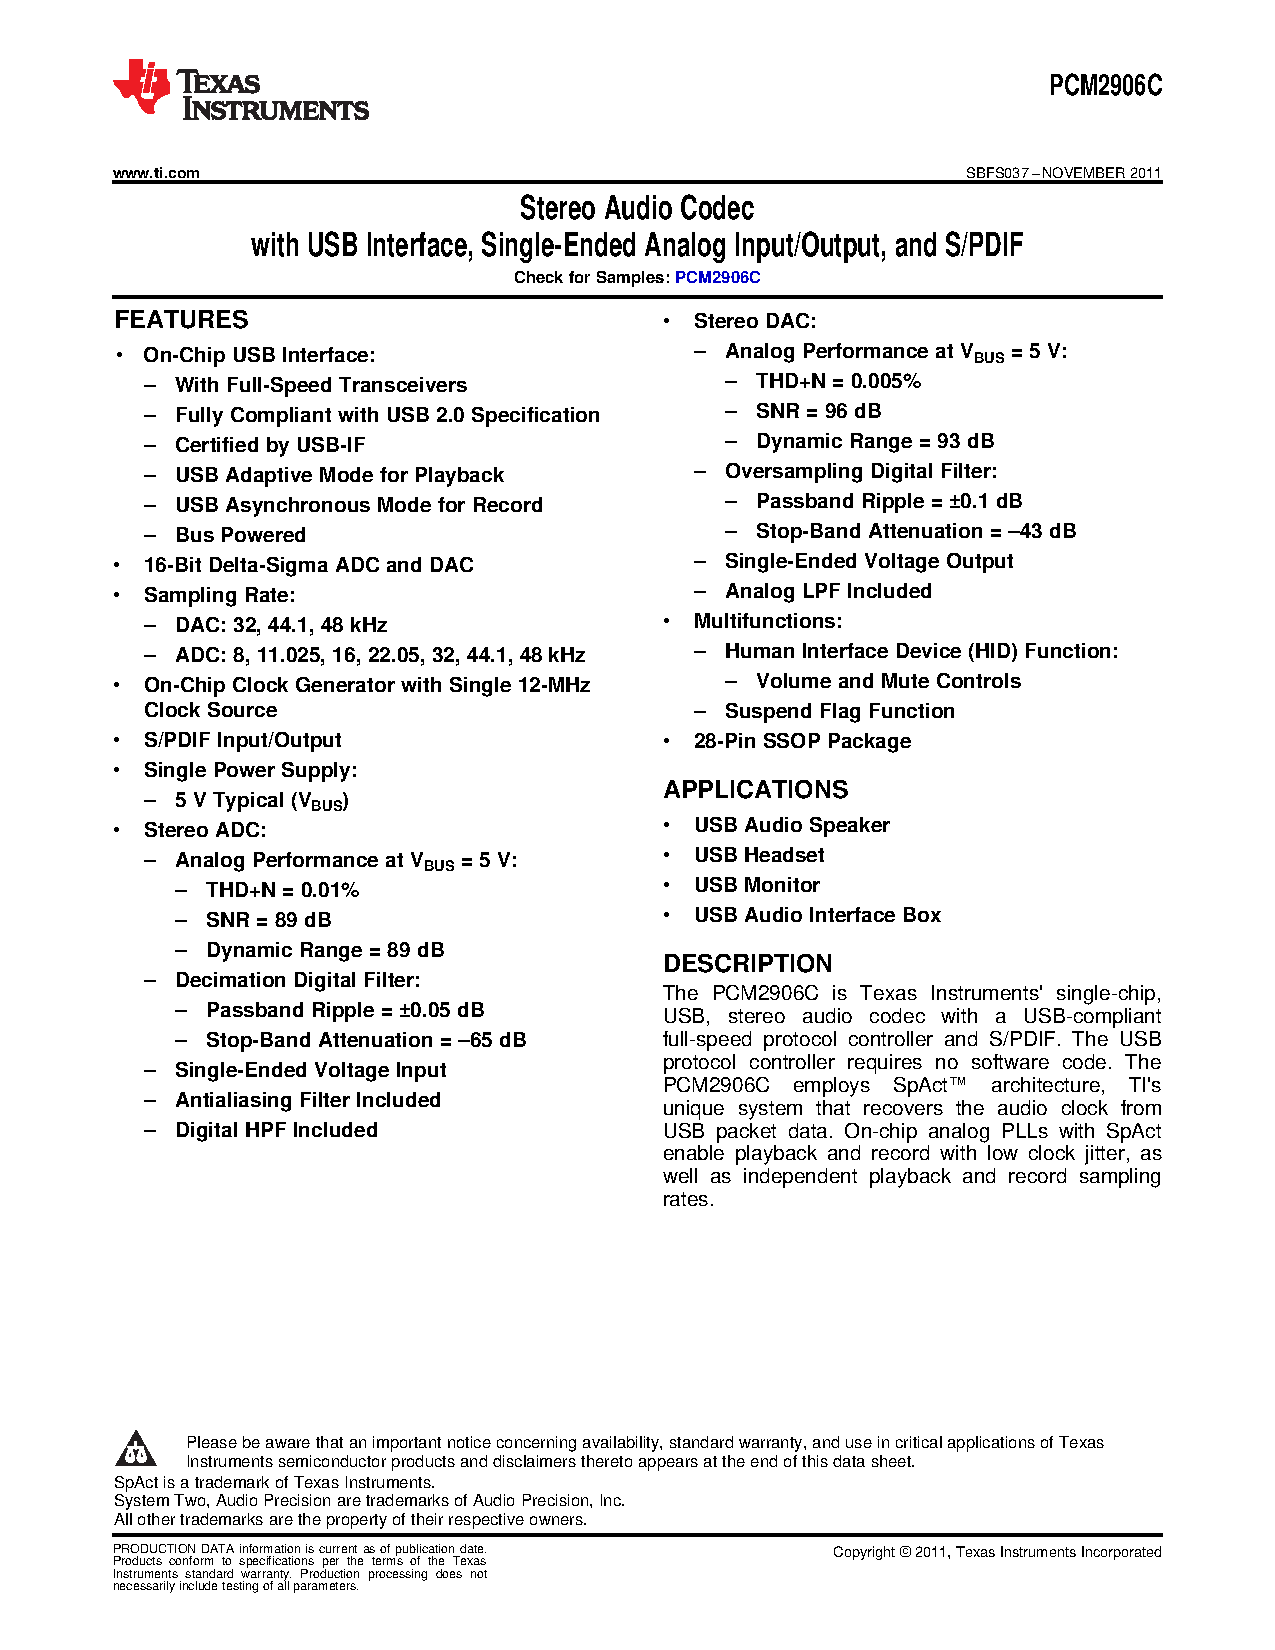
\includepdf[pages={1},noautoscale=false,fitpaper=false,pagecommand={\chapter{Datenblätter} \section{PCM2906C} \label{sec:pcm2906c} Link zum vollständigen Datenblatt \cite{data_PCM2906}},width=13cm]{datasheets/pcm2906c.pdf}
\includepdf[pages={2-4,7},noautoscale=false,fitpaper=false,width=1.1\textwidth, pagecommand={}]{datasheets/pcm2906c.pdf}

%%================ Abkuerzungsverzeichnis ==============%%
%% start of file abkuerzungen.tex

% Abkuerzungsverzeichnis
\addchap{
	\iflanguage{english}{Acronyms}{Abkürzungsverzeichnis}}
\begin{acronym}[ACRONYM]
\acro{acb}[ACB]{Audio-Connect-Box}
\acro{led}[LED]{light-emitting diode}
\acro{opv}[OPV]{Operationsverstärker}
\acro{rew}[REW]{Room EQ Wizard}
\acro{rfi}[RFI]{radio frequency interference}
\acro{pla}[PLA]{polylactic acid}
\end{acronym}\newpage

%% end of file abkuerzungen.tex
%%======================================================%%

%%================ Abbildungsverzeichnis ===============%%
\setcounter{lofdepth}{2}
\dipalistoffigures
%%======================================================%%

%%================ Tabellenverzeichnis  ================%%
\setcounter{lotdepth}{2}
\dipalistoftables
%%======================================================%%

%%================ Literaturverzeichnis ================%%
\newpage
%% start of file literatur.tex

%% Literaturverzeichnis:
\begin{Literatur}
% TODO nummerierung/reihenfolge literatur anpassen
\bibitem{data_PCM2906}{\textbf{TEXAS INSTRUMENTS:} \href{https://www.ti.com/lit/ds/symlink/pcm2906.pdf}{\emph{Datenblatt PCM2904/PCM2906}}. 2007 [online] 04.03.2022 Available: \url{https://www.ti.com/lit/ds/symlink/pcm2906.pdf}}

\bibitem{input}{\textbf{WHITLOCK, Bill:} \emph{A new balanced audio input circuit for maximum common-mode rejection in real-world environments}. Journal of the Audio Engineering Society, 1995, 43. Jg., Nr. 6, S. 454-464.}

\bibitem{phantom}{\textbf{PETROV, Petre Tzv:} \href{https://www.diyrecordingequipment.com/products/hc1}{\emph{5V DC To 48V DC Converter For Phantom Power Supplies}}. 04.03.2021, Electronicsforu. [online] 25.03.2022 https://www.electronicsforu.com/electronics-projects/5v-48v-dc-converter-phantom-power-supplies}

\bibitem{fachkunde}{\textbf{BUMILLER, Horst; et al:} {\emph{Fachkunde Elektrotechnik.}} Haan-Gruiten: Verlag Europa-Lehrmittel, Nourney, Vollmer GmbH \& Company KG, 2020. -ISBN 978-3-808-53791-6. S.} 

\bibitem{tietze} \textbf{U. TIETZE und C. SCHENK:} \textit{Electronic circuits. handbook for design and application.} Heidelberg: Springer, 2015.

\bibitem{litKomb} \textbf{Wikibooks:} (4.1.2021) \textit{LaTeX-Kompendium: Schnellkurs: Erstellen eines Literaturverzeichnisses}. [Online]. Available: \url{https://de.wikibooks.org/wiki/LaTeX-Kompendium:\_Schnellkurs:\_Erstellen\_eines\_Literaturverzeichnisses}


\end{Literatur}

%% end of file literatur.tex
%%======================================================%%


\end{document}
